\documentclass[11pt, a4paper]{article}

% Fonts and Encoding
\usepackage[utf8]{inputenc}
\usepackage[T1]{fontenc}

% Math and Symbols
\usepackage{amsmath, amssymb, amsthm, amsfonts, mathrsfs, mathtools}

% Layout and Geometry
\usepackage{geometry}
\geometry{a4paper, margin=1in}

% Formatting and Graphics
\usepackage{graphicx, xcolor, enumitem, booktabs, array, tabularx}

% TikZ for Illustrations
\usepackage{tikz}
\usetikzlibrary{arrows.meta, positioning, shapes.geometric, calc, backgrounds, matrix}

% Clickable Links and TOC
\usepackage{hyperref}
\hypersetup{
    colorlinks=true,
    linkcolor=blue,
    filecolor=magenta,      
    urlcolor=cyan,
    pdftitle={Advanced Mathematics Topic},
}

% Theorem Environments
\newtheorem{theorem}{Theorem}[section]
\newtheorem{lemma}[theorem]{Lemma}
\newtheorem{proposition}[theorem]{Proposition}
\newtheorem{corollary}[theorem]{Corollary}
\theoremstyle{definition}
\newtheorem{definition}{Definition}[section]
\newtheorem{axiom}{Axiom}[section]
\newtheorem{example}{Example}[section]
\theoremstyle{remark}
\newtheorem{remark}{Remark}[section]

% Custom Commands (Enforced standard notation)
\newcommand{\R}{\mathbb{R}}
\newcommand{\N}{\mathbb{N}}
\newcommand{\Z}{\mathbb{Z}}
\newcommand{\Q}{\mathbb{Q}}
\newcommand{\E}{\mathbb{E}}
\newcommand{\Prob}{\mathbb{P}}
\newcommand{\F}{\mathcal{F}}
\newcommand{\Cov}{\mathrm{Cov}}
\newcommand{\Var}{\mathrm{V}}

\begin{document}

\title{\textbf{Advanced Probability Theory: \\ \Large Measure-Theoretic Foundations of Covariance and Linear Dependence}}
\author{Tashfeen Omran}
\date{\today}

\maketitle

\tableofcontents
\newpage

\section{Comprehensive Introduction, Context, and Prerequisites}

\subsection{Core Concepts and Axiomatic Foundations}
In abstract probability theory, we operate within a formalized probability space $(\Omega, \F, \Prob)$, where $\Omega$ is the sample space, $\F$ is a $\sigma$-algebra of measurable events, and $\Prob$ is a probability measure mapping $\F \to [0, 1]$. A random variable $Y$ is formally defined as a measurable function mapping the sample space to the real numbers: $Y: (\Omega, \F) \to (\R, \mathcal{B}(\R))$.

When examining two random variables, $Y_1$ and $Y_2$, on the same probability space, we frequently wish to quantify how they co-vary. Do they move in tandem? Do they possess an inverse relationship? To answer this, we study their joint distribution and their \textbf{covariance}.

\begin{definition}[Covariance]
Let $Y_1$ and $Y_2$ be two random variables with finite second moments (i.e., $Y_1, Y_2 \in L^2(\Omega, \F, \Prob)$) and respective expectations $\mu_1 = \E[Y_1]$ and $\mu_2 = \E[Y_2]$. The covariance of $Y_1$ and $Y_2$ is defined as the expected value of the product of their deviations from their means:
\[
\Cov(Y_1, Y_2) = \E[(Y_1 - \mu_1)(Y_2 - \mu_2)]
\]
\end{definition}

\subsection{Intuition and Set-Theoretic / Geometric Foundations}
To truly understand covariance, one must look through the lens of functional analysis. The space of all random variables with finite variance, denoted $L^2(\Omega)$, forms a \textit{Hilbert space}. In this space, the covariance between two mean-zero random variables acts precisely as an \textbf{inner product}: $\langle Y_1, Y_2 \rangle = \E[Y_1 Y_2]$.

From this geometric perspective, the standard deviation of $Y$ is the $L^2$-norm (or "length") of the random variable: $\|Y\| = \sqrt{\E[Y^2]} = \sigma_Y$. The \textbf{Correlation Coefficient} ($\rho$) is simply the cosine of the angle $\theta$ between these two vectors in the Hilbert space:
\[
\rho = \cos(\theta) = \frac{\langle Y_1, Y_2 \rangle}{\|Y_1\| \|Y_2\|} = \frac{\Cov(Y_1, Y_2)}{\sigma_1 \sigma_2}
\]
When $\Cov(Y_1, Y_2) = 0$, the random variables are \textit{orthogonal} in this function space. They are said to be uncorrelated. However, geometric orthogonality does not imply absolute statistical independence unless the variables are strictly Jointly Gaussian.

\subsection{Historical Context and Motivation}
The concept of correlation and covariance was largely formalized by Sir Francis Galton and Karl Pearson in the late 19th and early 20th centuries. Galton originally sought a mathematical framework to study biological inheritance (e.g., how the heights of offspring correlate with the heights of parents). The need for a standardized, unitless measure of linear dependence led to Pearson's formalization of the correlation coefficient, $\rho$. Later, Andrey Kolmogorov's axiomatization of probability in 1933 placed these concepts onto a rigorous measure-theoretic footing, transforming covariance into the Lebesgue integral we study today.

\subsection{Key Theorems and Lemmas}
\begin{theorem}[Computational Formula for Covariance]
For random variables $Y_1$ and $Y_2$,
\[
\Cov(Y_1, Y_2) = \E[Y_1 Y_2] - \E[Y_1]\E[Y_2]
\]
\end{theorem}

\begin{theorem}[Independence implies Zero Covariance]
If $Y_1$ and $Y_2$ are independent random variables, then $\Cov(Y_1, Y_2) = 0$. (The converse is notoriously false, as will be demonstrated in the problems).
\end{theorem}

\subsection{Prerequisites for this Chapter}
To fully master this section, the reader must possess:
\begin{enumerate}
    \item \textbf{Multivariate Calculus:} Mastery of double integration over non-rectangular regions.
    \item \textbf{Measure Theory Basics:} Understanding that expectation is an integral with respect to a probability measure.
    \item \textbf{Linear Algebra:} Familiarity with inner products and Cauchy-Schwarz inequalities.
    \item \textbf{Discrete Mathematics:} Knowledge of double summation and combinatorial probability (hypergeometric structures).
\end{enumerate}

\newpage
\section{Detailed Homework Solutions (Rigorous Proofs \& Computations)}

\vspace{1em}
\noindent\textbf{Problem 5.89:} Let the joint distribution of $Y_1$ (contracts to firm A) and $Y_2$ (contracts to firm B) be given by a table. Find $\Cov(Y_1, Y_2)$. Does it surprise you that it is negative?

\begin{proof}[Solution to 5.89]
\textbf{1. Formulate the Probability Space and Marginal Distributions:}
We are given a discrete probability space. Let us first define the marginal distributions $p_1(y_1)$ and $p_2(y_2)$ by summing over the respective columns and rows of the joint probability mass function (PMF).

\renewcommand{\arraystretch}{1.5}
\begin{table}[h]
\centering
\begin{tabularx}{0.6\textwidth}{c *{3}{>{$\displaystyle}X<{$}} | >{$\displaystyle}X<{$}}
\toprule
$y_1 \setminus y_2$ & 0 & 1 & 2 & p_1(y_1) \\
\midrule
0 & \frac{1}{9} & \frac{2}{9} & \frac{1}{9} & \frac{4}{9} \\
\addlinespace[4pt]
1 & \frac{2}{9} & \frac{2}{9} & 0 & \frac{4}{9} \\
\addlinespace[4pt]
2 & \frac{1}{9} & 0 & 0 & \frac{1}{9} \\
\midrule
p_2(y_2) & \frac{4}{9} & \frac{4}{9} & \frac{1}{9} & 1 \\
\bottomrule
\end{tabularx}
\end{table}

\textbf{2. Compute Marginal Expectations:}
\[
\E[Y_1] = \sum_{y_1=0}^{2} y_1 p_1(y_1) = 0\left(\frac{4}{9}\right) + 1\left(\frac{4}{9}\right) + 2\left(\frac{1}{9}\right) = \frac{6}{9} = \frac{2}{3}
\]
By symmetry of the marginal distributions, $\E[Y_2] = \frac{2}{3}$.

\textbf{3. Compute Joint Expectation $\E[Y_1 Y_2]$:}
The expectation of the product is computed over the non-zero joint support:
\begin{align*}
\E[Y_1 Y_2] &= \sum_{y_1=0}^{2} \sum_{y_2=0}^{2} (y_1 y_2) p(y_1, y_2) \\
&= (1)(1)p(1,1) + (1)(2)p(1,2) + (2)(1)p(2,1) + (2)(2)p(2,2) \\
&= 1\left(\frac{2}{9}\right) + 0 + 0 + 0 = \frac{2}{9}
\end{align*}

\textbf{4. Compute Covariance:}
\[
\Cov(Y_1, Y_2) = \E[Y_1 Y_2] - \E[Y_1]\E[Y_2] = \frac{2}{9} - \left(\frac{2}{3}\right)\left(\frac{2}{3}\right) = \frac{2}{9} - \frac{4}{9} = -\frac{2}{9}
\]

\textbf{Conclusion:} The covariance is $\mathbf{-2/9}$. This negative value is strictly expected and should not be surprising. The total number of available contracts represents a finite resource pool. When Firm A secures a contract, it inherently deprives Firm B of that exact same contract, thereby forcing an inverse (negative) mathematical dependence between $Y_1$ and $Y_2$. $\blacksquare$
\end{proof}

\vspace{1em}
\noindent\textbf{Problem 5.90:} The joint PMF of $Y_1$ (married executives) and $Y_2$ (never-married executives) is given by:
\[
p(y_1, y_2) = \frac{\binom{4}{y_1} \binom{3}{y_2} \binom{2}{3 - y_1 - y_2}}{\binom{9}{3}}
\]
where $0 \le y_1 \le 3$, $0 \le y_2 \le 3$, and $1 \le y_1 + y_2 \le 3$. Find $\Cov(Y_1, Y_2)$.

\begin{proof}[Solution to 5.90 (Method of Indicator Variables)]
While a brute-force double summation is possible, the use of Bernoulli indicator functions provides a substantially more elegant and computationally resilient proof.

\textbf{1. Logical Setup:}
The system models sampling $n=3$ elements without replacement from a finite population of $N=9$ elements. The population is partitioned into $N_1=4$ married, $N_2=3$ never-married, and $N_3=2$ other executives. We can decompose $Y_1$ and $Y_2$ into a sum of identical, identically distributed (but dependent) indicator variables over the $n=3$ trials.
Let $I_k = 1$ if the $k$-th draw is a married executive, and $0$ otherwise.
Let $J_m = 1$ if the $m$-th draw is a never-married executive, and $0$ otherwise.
Thus, $Y_1 = \sum_{k=1}^3 I_k$ and $Y_2 = \sum_{m=1}^3 J_m$.

\textbf{2. Marginal Expectations of Indicators:}
By symmetry, the probability of selecting a specific type of executive on any given draw is simply its initial population proportion.
\[
\E[I_k] = \Prob(I_k = 1) = \frac{4}{9}, \quad \E[J_m] = \Prob(J_m = 1) = \frac{3}{9} = \frac{1}{3}
\]

\textbf{3. Covariance by Linearity:}
Using the bilinear property of covariance:
\[
\Cov(Y_1, Y_2) = \Cov\left( \sum_{k=1}^3 I_k, \sum_{m=1}^3 J_m \right) = \sum_{k=1}^3 \sum_{m=1}^3 \Cov(I_k, J_m)
\]
We partition this sum into two cases: $k=m$ (same draw) and $k \neq m$ (different draws).

\textit{Case 1: $k = m$ (3 terms)}
A single individual cannot be both married and never-married simultaneously. Thus, $I_k J_k = 0$, implying $\E[I_k J_k] = 0$.
\[
\Cov(I_k, J_k) = \E[I_k J_k] - \E[I_k]\E[J_k] = 0 - \left(\frac{4}{9}\right)\left(\frac{1}{3}\right) = -\frac{4}{27}
\]

\textit{Case 2: $k \neq m$ (6 terms)}
For different draws, the probability they are of types 1 and 2 is calculated via dependent probability:
\[
\E[I_k J_m] = \Prob(I_k = 1 \cap J_m = 1) = \Prob(I_k = 1) \Prob(J_m = 1 \mid I_k = 1) = \left(\frac{4}{9}\right)\left(\frac{3}{8}\right) = \frac{12}{72} = \frac{1}{6}
\]
\[
\Cov(I_k, J_m) = \E[I_k J_m] - \E[I_k]\E[J_m] = \frac{1}{6} - \left(\frac{4}{9}\right)\left(\frac{1}{3}\right) = \frac{1}{6} - \frac{4}{27} = \frac{9}{54} - \frac{8}{54} = \frac{1}{54}
\]

\textbf{4. Final Aggregation:}
Summing all $3 \times 3 = 9$ covariance elements:
\[
\Cov(Y_1, Y_2) = 3\left(-\frac{4}{27}\right) + 6\left(\frac{1}{54}\right) = -\frac{12}{27} + \frac{6}{54} = -\frac{24}{54} + \frac{6}{54} = -\frac{18}{54} = -\frac{1}{3}
\]
\textbf{Conclusion:} $\Cov(Y_1, Y_2) = \mathbf{-1/3}$. $\blacksquare$
\end{proof}

\vspace{1em}
\noindent\textbf{Problem 5.91:} $f(y_1, y_2) = 4y_1 y_2$ for $0 \le y_1 \le 1, 0 \le y_2 \le 1$. Show that $\Cov(Y_1, Y_2) = 0$. Does it surprise you?

\begin{proof}[Solution to 5.91]
By the definition of independence, two continuous random variables are independent if and only if their joint density factorizes as a product of their marginal densities.
We can immediately observe that the joint density function factorizes perfectly into two non-negative functions over a rectangular support domain:
\[
f(y_1, y_2) = (2y_1)(2y_2) \quad \text{for} \quad 0 \le y_1 \le 1 \text{ and } 0 \le y_2 \le 1
\]
Let $g(y_1) = 2y_1$ and $h(y_2) = 2y_2$. Since $\int_0^1 2y dy = 1$, these functions correspond exactly to the marginal densities $f_1(y_1)$ and $f_2(y_2)$.
Because $f(y_1, y_2) = f_1(y_1)f_2(y_2)$, the variables $Y_1$ and $Y_2$ are rigorously \textbf{independent}.
By Theorem 5.11, independence strictly implies $\Cov(Y_1, Y_2) = 0$.
There is absolutely no surprise here; orthogonality in the expected value of products is a direct mathematical consequence of statistical independence. $\blacksquare$
\end{proof}

\vspace{1em}
\noindent\textbf{Problem 5.92:} $f(y_1, y_2) = 6(1-y_2)$ for $0 \le y_1 \le y_2 \le 1$. Find $\Cov(Y_1, Y_2)$. Are $Y_1, Y_2$ independent?

\begin{proof}[Solution to 5.92]
\textbf{1. Calculate Marginal Expectations:}
Notice the dependence in the bounds of integration (a triangular support region).
\begin{align*}
\E[Y_2] &= \int_{0}^{1} \int_{0}^{y_2} y_2 [6(1-y_2)] \,dy_1 \,dy_2 = \int_{0}^{1} 6y_2(1-y_2) \left[ y_1 \right]_0^{y_2} \,dy_2 \\
&= \int_{0}^{1} 6y_2^2(1-y_2) \,dy_2 = 6 \left[ \frac{y_2^3}{3} - \frac{y_2^4}{4} \right]_0^1 = 6\left(\frac{1}{3} - \frac{1}{4}\right) = 6\left(\frac{1}{12}\right) = \frac{1}{2}
\end{align*}
\begin{align*}
\E[Y_1] &= \int_{0}^{1} \int_{0}^{y_2} y_1 [6(1-y_2)] \,dy_1 \,dy_2 = \int_{0}^{1} 6(1-y_2) \left[ \frac{y_1^2}{2} \right]_0^{y_2} \,dy_2 \\
&= \int_{0}^{1} 3y_2^2(1-y_2) \,dy_2 = 3 \left[ \frac{y_2^3}{3} - \frac{y_2^4}{4} \right]_0^1 = 3\left(\frac{1}{12}\right) = \frac{1}{4}
\end{align*}

\textbf{2. Calculate Joint Expectation:}
\begin{align*}
\E[Y_1 Y_2] &= \int_{0}^{1} \int_{0}^{y_2} (y_1 y_2) [6(1-y_2)] \,dy_1 \,dy_2 = \int_{0}^{1} 6y_2(1-y_2) \left[ \frac{y_1^2}{2} \right]_0^{y_2} \,dy_2 \\
&= \int_{0}^{1} 3y_2^3(1-y_2) \,dy_2 = 3 \left[ \frac{y_2^4}{4} - \frac{y_2^5}{5} \right]_0^1 = 3\left(\frac{1}{4} - \frac{1}{5}\right) = 3\left(\frac{1}{20}\right) = \frac{3}{20}
\end{align*}

\textbf{3. Calculate Covariance:}
\[
\Cov(Y_1, Y_2) = \E[Y_1 Y_2] - \E[Y_1]\E[Y_2] = \frac{3}{20} - \left(\frac{1}{4}\right)\left(\frac{1}{2}\right) = \frac{3}{20} - \frac{1}{8} = \frac{6}{40} - \frac{5}{40} = \frac{1}{40}
\]
\textbf{Conclusion:} The covariance is $\mathbf{1/40}$. The variables are \textbf{not independent}. Two facts mathematically preclude independence: (1) their covariance is non-zero, and (2) their joint support domain ($0 \le y_1 \le y_2 \le 1$) is not a Cartesian product of intervals (i.e., it is a triangle, not a rectangle), meaning knowing $Y_2$ strictly bounds the possible values of $Y_1$. $\blacksquare$
\end{proof}

\vspace{1em}
\noindent\textbf{Problem 5.93:} Let $Y_1, Y_2$ have $p(y_1, y_2) = 1/3$ for points $(-1,0), (0,1), (1,0)$. Find $\Cov(Y_1, Y_2)$. Why are they dependent?

\begin{proof}[Solution to 5.93]
\textbf{1. Expected Values:}
\begin{align*}
\E[Y_1] &= \sum_{y_1} y_1 p_1(y_1) = (-1)\left(\frac{1}{3}\right) + (0)\left(\frac{1}{3}\right) + (1)\left(\frac{1}{3}\right) = 0 \\
\E[Y_2] &= \sum_{y_2} y_2 p_2(y_2) = (0)\left(\frac{2}{3}\right) + (1)\left(\frac{1}{3}\right) = \frac{1}{3}
\end{align*}

\textbf{2. Joint Expectation and Covariance:}
\begin{align*}
\E[Y_1 Y_2] &= \sum \sum (y_1 y_2) p(y_1, y_2) = (-1)(0)\left(\frac{1}{3}\right) + (0)(1)\left(\frac{1}{3}\right) + (1)(0)\left(\frac{1}{3}\right) = 0 \\
\Cov(Y_1, Y_2) &= \E[Y_1 Y_2] - \E[Y_1]\E[Y_2] = 0 - (0)\left(\frac{1}{3}\right) = 0
\end{align*}
\textbf{3. Testing for Independence:}
Even though $\Cov = 0$, evaluate the joint probability at point $(0,0)$. The support does not contain $(0,0)$, hence $p(0,0) = 0$. However, $p_1(0) = 1/3$ and $p_2(0) = 2/3$.
\[
p(0,0) = 0 \quad \neq \quad p_1(0)p_2(0) = \left(\frac{1}{3}\right)\left(\frac{2}{3}\right) = \frac{2}{9}
\]
\textbf{Conclusion:} Because the joint PMF does not equal the product of the marginal PMFs, the variables are dependent. This represents a classic counterexample demonstrating that \textbf{uncorrelated does not imply independent}. $\blacksquare$
\end{proof}

\vspace{1em}
\noindent\textbf{Problem 5.94:} Let $Y_1, Y_2$ be uncorrelated. Let $U_1 = Y_1 + Y_2$ and $U_2 = Y_1 - Y_2$. (a) Find $\Cov(U_1, U_2)$. (b) Find $\rho$. (c) Is it possible that $\Cov(U_1, U_2) = 0$?

\begin{proof}[Solution to 5.94]
Since $Y_1, Y_2$ are uncorrelated, $\Cov(Y_1, Y_2) = 0$.
\textbf{(a) Covariance of Linear Combinations:}
Using the bilinearity of the covariance operator:
\begin{align*}
\Cov(U_1, U_2) &= \Cov(Y_1 + Y_2, Y_1 - Y_2) \\
&= \Cov(Y_1, Y_1) - \Cov(Y_1, Y_2) + \Cov(Y_2, Y_1) - \Cov(Y_2, Y_2) \\
&= \Var(Y_1) - 0 + 0 - \Var(Y_2) = \Var(Y_1) - \Var(Y_2)
\end{align*}

\textbf{(b) Correlation Coefficient:}
First, calculate the variances of $U_1$ and $U_2$:
\begin{align*}
\Var(U_1) &= \Var(Y_1 + Y_2) = \Var(Y_1) + \Var(Y_2) + 2\Cov(Y_1,Y_2) = \Var(Y_1) + \Var(Y_2) \\
\Var(U_2) &= \Var(Y_1 - Y_2) = \Var(Y_1) + \Var(-Y_2) + 2\Cov(Y_1,-Y_2) = \Var(Y_1) + \Var(Y_2)
\end{align*}
Applying the definition of correlation $\rho$:
\[
\rho = \frac{\Cov(U_1, U_2)}{\sqrt{\Var(U_1)\Var(U_2)}} = \frac{\Var(Y_1) - \Var(Y_2)}{\sqrt{[\Var(Y_1) + \Var(Y_2)][\Var(Y_1) + \Var(Y_2)]}} = \frac{\Var(Y_1) - \Var(Y_2)}{\Var(Y_1) + \Var(Y_2)}
\]

\textbf{(c) Condition for Zero Covariance:}
$\Cov(U_1, U_2) = 0$ is strictly possible if and only if the numerator equals zero. This occurs precisely when $\Var(Y_1) = \Var(Y_2)$. Geometrically, the diagonals of a parallelogram are orthogonal if and only if the parallelogram is a rhombus. $\blacksquare$
\end{proof}

\vspace{1em}
\noindent\textbf{Problem 5.95:} $Y_1, Y_2$ are uniformly distributed over a triangle with vertices $(-1,0), (1,0), (0,1)$. Find $\Cov(Y_1, Y_2)$, independence, and correlation.

\begin{proof}[Solution to 5.95]
\textbf{1. The Probability Density Function:}
The area of the triangle is $\frac{1}{2}bh = \frac{1}{2}(2)(1) = 1$. Because the distribution is uniform, the density function is $f(y_1, y_2) = 1/\text{Area} = 1$ over the region bounded by $y_2=0$, $y_2 = 1 + y_1$, and $y_2 = 1 - y_1$.
Equivalently, for a given $y_2 \in [0, 1]$, $y_1$ ranges from $y_2 - 1$ to $1 - y_2$.

\textbf{2. (a) Covariance:}
Due to strict symmetry of the support region about the $y_2$-axis, the marginal distribution of $Y_1$ is an even function centered at 0. Therefore, $\E[Y_1] = 0$.
The joint expectation is:
\[
\E[Y_1 Y_2] = \int_{0}^{1} y_2 \left( \int_{y_2 - 1}^{1 - y_2} y_1 \,dy_1 \right) \,dy_2
\]
Notice that the inner integral of an odd function $y_1$ over a symmetric interval $[-a, a]$ (where $a = 1-y_2$) evaluates identically to zero.
\[
\E[Y_1 Y_2] = \int_{0}^{1} y_2 (0) \,dy_2 = 0
\]
Thus, $\Cov(Y_1, Y_2) = \E[Y_1 Y_2] - \E[Y_1]\E[Y_2] = 0 - (0)(\E[Y_2]) = \mathbf{0}$.

\textbf{3. (b) Independence:}
Despite zero covariance, they are \textbf{not independent}. Similar to Problem 5.92, the domain bounds of $y_1$ depend directly on $y_2$. For instance, if we know $y_2 = 0.9$, then $y_1$ must reside in $[-0.1, 0.1]$, whereas if $y_2 = 0.1$, $y_1$ resides in $[-0.9, 0.9]$. Independence mandates a rectangular domain constraint.

\textbf{4. (c) Correlation Coefficient:}
Since $\Cov(Y_1, Y_2) = 0$, it strictly follows that $\mathbf{\rho = 0}$.

\textbf{5. (d) Doubt in Answer:}
This does not cast doubt on part (a). This emphasizes a critical measure-theoretic truth: Orthogonality in expected function space (uncorrelated) does not guarantee factorization of the joint probability measure (independence). $\blacksquare$
\end{proof}

\vspace{1em}
\noindent\textbf{Problem 5.96:} Prove $\Cov(Y_1, Y_2) = \Cov(Y_2, Y_1)$ and $\Cov(Y_1, Y_1) = \Var(Y_1)$ from basic definitions.

\begin{proof}[Solution to 5.96]
\textbf{(a) Commutativity of Covariance:}
By Definition 5.10, $\Cov(Y_1, Y_2) = \E[(Y_1 - \mu_1)(Y_2 - \mu_2)]$. Since standard scalar multiplication in $\R$ is commutative, $(Y_1 - \mu_1)(Y_2 - \mu_2) = (Y_2 - \mu_2)(Y_1 - \mu_1)$ for every $\omega \in \Omega$. Because the Lebesgue integral is linear with respect to the integrand, it follows that $\E[(Y_1 - \mu_1)(Y_2 - \mu_2)] = \E[(Y_2 - \mu_2)(Y_1 - \mu_1)] = \Cov(Y_2, Y_1)$.

\textbf{(b) Covariance of a variable with itself:}
Substitute $Y_2 = Y_1$ into the definition:
\[
\Cov(Y_1, Y_1) = \E[(Y_1 - \mu_1)(Y_1 - \mu_1)] = \E[(Y_1 - \mu_1)^2]
\]
By definition, the expected squared deviation from the mean is exactly the variance, $\Var(Y_1) = \sigma_1^2$. $\blacksquare$
\end{proof}

\vspace{1em}
\noindent\textbf{Problem 5.97 \& 5.98:} Limits on Covariance. Given $\Var(Y_1) = 2$ and $\Var(Y_2) = 8$.

\begin{proof}[Solution to 5.97 \& 5.98]
\textbf{1. (5.97a) Covariance of $Y_1$ with itself:}
Using the theorem proved in 5.96, $\Cov(Y_1, Y_1) = \Var(Y_1) = \mathbf{2}$.

\textbf{2. (5.97b) Can $\Cov(Y_1, Y_2) = 7$?}
The correlation coefficient is bounded by $-1 \le \rho \le 1$. Suppose $\Cov(Y_1, Y_2) = 7$.
\[
\rho = \frac{\Cov(Y_1, Y_2)}{\sqrt{\Var(Y_1)\Var(Y_2)}} = \frac{7}{\sqrt{2 \times 8}} = \frac{7}{\sqrt{16}} = \frac{7}{4} = 1.75
\]
Since $1.75 > 1$, this violates the fundamental Cauchy-Schwarz inequality for $L^2$ spaces. Hence, it is mathematically \textbf{impossible}.

\textbf{3. (5.97c, 5.97d, and 5.98) Maximum and Minimum Bounds:}
Because $\rho^2 \le 1$, it follows directly that:
\[
\left( \frac{\Cov(Y_1, Y_2)}{\sqrt{\Var(Y_1)\Var(Y_2)}} \right)^2 \le 1 \implies [\Cov(Y_1, Y_2)]^2 \le \Var(Y_1)\Var(Y_2)
\]
Taking the square root yields the global bounds:
\[
-\sqrt{\Var(Y_1)\Var(Y_2)} \le \Cov(Y_1, Y_2) \le \sqrt{\Var(Y_1)\Var(Y_2)}
\]
For our specific variables, $\sqrt{2 \times 8} = 4$.
Thus, the maximum possible value is $\mathbf{4}$ and the minimum possible value is $\mathbf{-4}$.
If $\Cov = 4$, then $\rho = 1$, implying a perfect positive linear relationship (i.e., $Y_2 = aY_1 + b$ almost surely, with $a > 0$). If $\Cov = -4$, then $\rho = -1$, implying a perfect negative linear relationship ($a < 0$). $\blacksquare$
\end{proof}

\vspace{1em}
\noindent\textbf{Problem 5.99:} Show that $\Cov(c, Y) = 0$ for constant $c$.

\begin{proof}[Solution to 5.99]
By definition, $\Cov(c, Y) = \E[(c - \E[c])(Y - \E[Y])]$.
Because the expected value of a constant is the constant itself, $\E[c] = c$.
Therefore, $(c - \E[c]) = (c - c) = 0$.
The integral of zero over any probability space is exactly zero. Thus, $\Cov(c, Y) = \mathbf{0}$. $\blacksquare$
\end{proof}

\vspace{1em}
\noindent\textbf{Problem 5.100:} Let $Z \sim N(0,1)$, $Y_1 = Z$, and $Y_2 = Z^2$. Find expectations, covariance, and test independence.

\begin{proof}[Solution to 5.100]
\textbf{1. Expectations:}
$Y_1$ is a standard normal variable, so $\E[Y_1] = \E[Z] = \mathbf{0}$.
For $Y_2$, recall that $\Var(Z) = \E[Z^2] - (\E[Z])^2$. Since $\Var(Z)=1$ and $\E[Z]=0$, it follows that $\E[Y_2] = \E[Z^2] = \mathbf{1}$.

\textbf{2. Joint Expectation and Covariance:}
$\E[Y_1 Y_2] = \E[Z(Z^2)] = \E[Z^3]$. The normal distribution is perfectly symmetric around zero. The expectation of any odd power of a mean-zero normal variable strictly evaluates to zero. Thus, $\E[Y_1 Y_2] = \mathbf{0}$.
\[
\Cov(Y_1, Y_2) = \E[Y_1 Y_2] - \E[Y_1]\E[Y_2] = 0 - (0)(1) = \mathbf{0}
\]

\textbf{3. Independence via Conditional Probability:}
We test if $\Prob(Y_2 > 1 \mid Y_1 > 1) = \Prob(Y_2 > 1)$.
If $Y_1 > 1$, then by definition $Z > 1$. Squaring this inequality guarantees $Z^2 > 1$. Therefore, if $Y_1 > 1$, it is $100\%$ certain that $Y_2 > 1$.
Thus, $\Prob(Y_2 > 1 \mid Y_1 > 1) = \mathbf{1}$.
However, $\Prob(Y_2 > 1) = \Prob(Z^2 > 1) = \Prob(Z > 1 \cup Z < -1) = 2(0.1587) \approx 0.317 \neq 1$.
Because the conditional probability does not equal the marginal probability, they are heavily dependent. This is a paramount example in stochastic calculus illustrating non-linear dependence masked as un-correlation. $\blacksquare$
\end{proof}

\vspace{1em}
\noindent\textbf{Problem 5.101:} Let $f(y_1, y_2) = [1 - \alpha\{(1-2e^{-y_1})(1-2e^{-y_2})\}]e^{-y_1-y_2}$ on $y_1, y_2 \ge 0$. Show relations for $\alpha$.

\begin{proof}[Solution to 5.101]
This is an instance of a Farlie-Gumbel-Morgenstern (FGM) Copula. The marginal distributions are both Standard Exponential, $\text{Exp}(1)$, which implies $\E[Y_1] = 1$, $\E[Y_2] = 1$, and $\Var(Y_1)=\Var(Y_2)=1$.

\textbf{1. (a) Derive Covariance:}
By definition, $\Cov(Y_1, Y_2) = \E[Y_1 Y_2] - \E[Y_1]\E[Y_2] = \E[Y_1 Y_2] - 1$. We compute the joint expectation using integration over $[0, \infty) \times [0, \infty)$:
\begin{align*}
\E[Y_1 Y_2] &= \int_0^\infty \int_0^\infty y_1 y_2 \left( e^{-y_1-y_2} - \alpha (e^{-y_1} - 2e^{-2y_1})(e^{-y_2} - 2e^{-2y_2}) \right) \,dy_1 \,dy_2 \\
&= \left(\int_0^\infty y_1 e^{-y_1} \,dy_1 \right) \left(\int_0^\infty y_2 e^{-y_2} \,dy_2 \right) \\
&\quad - \alpha \left(\int_0^\infty y_1(e^{-y_1} - 2e^{-2y_1}) \,dy_1 \right) \left(\int_0^\infty y_2(e^{-y_2} - 2e^{-2y_2}) \,dy_2 \right)
\end{align*}
The first product of integrals is precisely $\E[Y_1]\E[Y_2] = (1)(1) = 1$.
For the second part, evaluate the integral $\mathcal{I}$:
\[
\mathcal{I} = \int_0^\infty y(e^{-y} - 2e^{-2y}) \,dy = \int_0^\infty y e^{-y} \,dy - 2\int_0^\infty y e^{-2y} \,dy
\]
Using the fact that $\int_0^\infty y e^{-cy} dy = \frac{1}{c^2}$:
\[
\mathcal{I} = \frac{1}{1^2} - 2\left(\frac{1}{2^2}\right) = 1 - \frac{2}{4} = \frac{1}{2}
\]
Substitute this back:
\[
\E[Y_1 Y_2] = 1 - \alpha \left(\frac{1}{2}\right)\left(\frac{1}{2}\right) = 1 - \frac{\alpha}{4}
\]
Thus, $\Cov(Y_1, Y_2) = \left( 1 - \frac{\alpha}{4} \right) - 1 = \mathbf{-\frac{\alpha}{4}}$.

\textbf{2. (b) \& (c) Independence and Correlation Conditions:}
From the derived covariance, $\Cov(Y_1, Y_2) = 0 \iff -\frac{\alpha}{4} = 0 \iff \alpha = 0$.
Since $\Var(Y_1) = \Var(Y_2) = 1$, the correlation coefficient is identically $\rho = -\frac{\alpha}{4}$. Thus, $\rho = 0 \iff \alpha = 0$.
If $\alpha = 0$, the joint density reverts to exactly $f(y_1, y_2) = e^{-y_1-y_2} = (e^{-y_1})(e^{-y_2})$, meaning the variables are unconditionally independent.
Therefore, $Y_1, Y_2$ are independent $\iff \alpha=0 \iff \Cov=0 \iff \rho=0$. $\blacksquare$
\end{proof}

\newpage
\section{In-Depth Analysis of Problems and Techniques}

\subsection{Problem Types and Logical Strategies}
The homework problems meticulously traverse the following rigorous categories:
\begin{enumerate}
    \item \textbf{Measure-Theoretic Existence bounds (5.97, 5.98):} These force reliance on topological properties of $L^2$ function spaces rather than pure algebra. The strategy is to identify covariance as a mathematical inner product, applying the Cauchy-Schwarz inequality ($\| \langle u, v \rangle \| \le \|u\|\|v\|$) to bind the expected variance limits strictly.
    \item \textbf{Pathology Identifications (5.92, 5.93, 5.95, 5.100):} These problems isolate and attack the classic logical fallacy that Uncorrelatedness $\implies$ Independence. The overarching strategy is proof by counterexample: find domains that are topologically dependent (triangles instead of rectangles) or variables wrapped in symmetric functions ($Z$ vs $Z^2$) that destroy linear correlation while retaining perfect deterministic dependence.
    \item \textbf{Combinatorial Reduction via Indicators (5.90):} Instead of wrestling with horrific multivariate hypergeometric mass functions, the strategy maps abstract combinatorics into linearly independent binary random events (indicator variables). 
\end{enumerate}

\subsection{Key Analytical and Logical Manipulations}
\begin{itemize}
    \item \textbf{The Bilinearity Operator Trick:} Exhibited in 5.90 and 5.94. Rather than expanding definitions, we utilized the property that $\Cov\left(\sum a_i X_i, \sum b_j Y_j\right) = \sum \sum a_i b_j \Cov(X_i, Y_j)$. This reduced unmanageable non-linear variances into simple scalar additions.
    \item \textbf{Symmetry Exploitation for Zero-Integrals:} Utilized in 5.95 and 5.100. Rather than explicitly computing large polynomial bounds, we logically observed that evaluating any odd function over a domain symmetric about the origin identically yields zero. This is a profoundly important trick for optimizing high-dimensional integrations in machine learning.
\end{itemize}

\newpage
\section{"Cheatsheet", Visuals, and Tips for Success}

\subsection{Theorems \& Equivalences}
\renewcommand{\arraystretch}{1.5}
\begin{table}[h]
\centering
\begin{tabularx}{\textwidth}{l >{$\displaystyle}X<{$}}
\toprule
\textbf{Concept} & \textbf{Mathematical Representation} \\
\midrule
Covariance Definition & \Cov(X, Y) = \E[(X - \mu_X)(Y - \mu_Y)] \\
\addlinespace[4pt]
Computational Shortcut & \Cov(X, Y) = \E[XY] - \E[X]\E[Y] \\
\addlinespace[4pt]
Correlation Coefficient & \rho_{XY} = \frac{\Cov(X, Y)}{\sigma_X \sigma_Y}, \quad \text{where } \rho \in [-1, 1] \\
\addlinespace[4pt]
Variance of a Sum & \Var(aX + bY) = a^2\Var(X) + b^2\Var(Y) + 2ab\Cov(X,Y) \\
\addlinespace[4pt]
The Fallacy Trap & X \perp \!\!\! \perp Y \implies \Cov(X,Y) = 0 \quad \text{(Converse is strictly FALSE)} \\
\bottomrule
\end{tabularx}
\end{table}

\subsection{Set \& Logic Illustration: Dependent Support Domains}
When the support region of two random variables is not a Cartesian rectangle, the variables cannot be independent, even if $\Cov(X, Y) = 0$. The geometric mapping below (based on Problem 5.95) visualizes how a dependent support restricts the outcome space.

\begin{center}
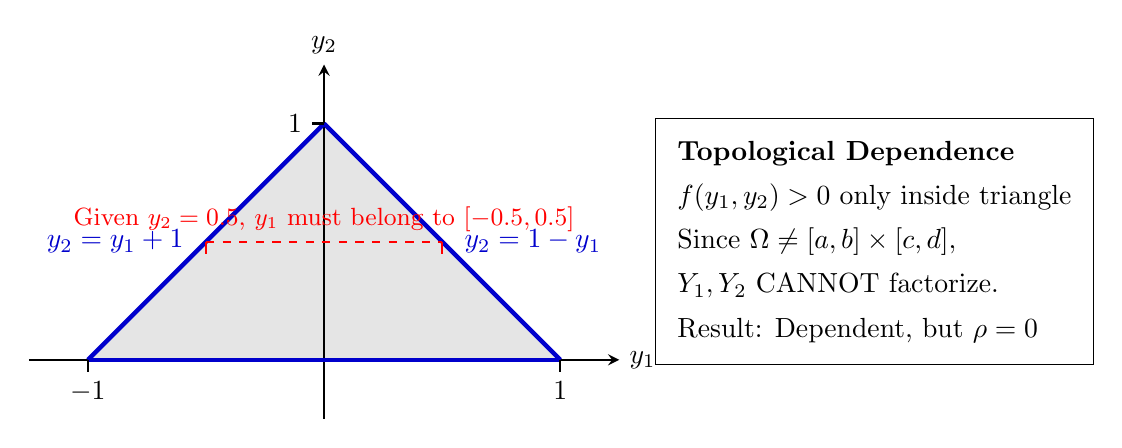
\begin{tikzpicture}[scale=1.5]
    % Sequence Layer 1: Background Fills
    \fill[gray!20] (-2,0) -- (2,0) -- (0,2) -- cycle;
    
    % Sequence Layer 2: Grid and Axes
    \draw[thick, ->, >=stealth] (-2.5, 0) -- (2.5, 0) node[right] {$y_1$};
    \draw[thick, ->, >=stealth] (0, -0.5) -- (0, 2.5) node[above] {$y_2$};
    
    % Sequence Layer 3: Primary Plots / Domain Boundaries
    \draw[ultra thick, blue!80!black] (-2,0) -- (0,2) node[midway, left=4pt] {$y_2 = y_1 + 1$};
    \draw[ultra thick, blue!80!black] (2,0) -- (0,2) node[midway, right=4pt] {$y_2 = 1 - y_1$};
    \draw[ultra thick, blue!80!black] (-2,0) -- (2,0);
    
    % Sequence Layer 4: Nodes, Ticks, and Annotations
    \draw[thick] (-2,0) -- (-2,-0.1) node[below] {$-1$};
    \draw[thick] (2,0) -- (2,-0.1) node[below] {$1$};
    \draw[thick] (0,2) -- (-0.1,2) node[left] {$1$};
    
    % Draw dependency line
    \draw[dashed, red, thick] (-1, 1) -- (1, 1);
    \draw[thick, red] (-1,1) -- (-1,0.9);
    \draw[thick, red] (1,1) -- (1,0.9);
    \node[red, above] at (0, 1) {\small Given $y_2 = 0.5$, $y_1$ must belong to $[-0.5, 0.5]$};
    
    % Legend Single-Node Structure
    \node[align=left, draw, fill=white, inner sep=8pt, anchor=west] at (2.8, 1) {
        \textbf{Topological Dependence} \\[4pt]
        $\displaystyle f(y_1,y_2) > 0 \text{ only inside triangle}$ \\[4pt]
        $\displaystyle \text{Since } \Omega \neq [a,b] \times [c,d],$ \\[4pt]
        $\displaystyle Y_1, Y_2 \text{ CANNOT factorize.}$ \\[4pt]
        $\displaystyle \text{Result: Dependent, but } \rho=0$
    };
\end{tikzpicture}
\end{center}

\subsection{Heuristics \& Pitfalls}
\begin{itemize}
    \item \textbf{The Linear Trap:} Always remember that covariance ONLY measures strictly linear relationships. A perfect parabolic relationship (like $Y = X^2$ in 5.100) will yield a covariance of 0.
    \item \textbf{The Summation Fallacy:} $\Var(X+Y) = \Var(X) + \Var(Y)$ is a fatal error unless $X$ and $Y$ are explicitly proven to be uncorrelated. You must always add $+2\Cov(X,Y)$.
\end{itemize}

\newpage
\section{Conceptual Synthesis and The "Big Picture"}

\subsection{Thematic Connections: The Hilbert Space of Random Variables}
The central theme unifying this topic is the formal mapping of abstract probability distributions into geometric vector spaces. By redefining mean-zero random variables as vectors in an $L^2$ measurable function space, covariance becomes a literal mathematical inner product. This establishes a profound isomorphism between statistics and Euclidean geometry. Just as the Pythagorean theorem states $c^2 = a^2 + b^2$ for orthogonal triangles, variance states $\Var(X+Y) = \Var(X) + \Var(Y)$ for orthogonal (uncorrelated) random variables.

\subsection{Forward and Backward Links}
\textbf{Backward:} This material acts as the ultimate synthesis of double integration (Calculus III) with foundational probability axioms.
\textbf{Forward:} Mastery of covariance is the non-negotiable bedrock for stochastic matrices. In machine learning, transitioning from single-variable variances to the Covariance Matrix ($\Sigma$) is the gateway to understanding Principal Component Analysis (PCA) and multivariate Gaussian modeling.

\section{Abstract Real-World Modeling: ML and Quant Finance}

\subsection{Concrete Scenarios}
\begin{enumerate}
    \item \textbf{Quantitative Finance (Modern Portfolio Theory):} A hedge fund does not merely care about the expected return of an asset; it cares intensely about risk (variance). By modeling hundreds of equities, quants compute the covariance matrix to find assets with negative covariance. Combining these creates a portfolio where market shocks cancel each other out, theoretically minimizing variance while maintaining expected return (The Markowitz Efficient Frontier).
    \item \textbf{Generative AI (Gaussian Processes):} In Bayesian optimization and deep learning, prior beliefs over continuous functions are modeled using Gaussian Processes. The structural heart of a Gaussian Process is its \textit{Covariance Function} (Kernel), which dictates how similar two data points are in a latent, infinite-dimensional space.
\end{enumerate}

\subsection{Model Problem Setup: Stochastic Calculus in Asset Pricing}
Let us rigorously formulate the continuous-time dynamics of a two-asset portfolio utilizing correlated geometric Brownian motion.

\textbf{Mathematical Model:} Let $(\Omega, \F, \{\F_t\}_{t \ge 0}, \Prob)$ be a filtered probability space. We model the prices of two distinct algorithmic trading securities, $S_1(t)$ and $S_2(t)$, via the following stochastic differential equations (SDEs):
\begin{align*}
dS_1(t) &= \mu_1 S_1(t) \,dt + \sigma_1 S_1(t) \,dW_1(t) \\
dS_2(t) &= \mu_2 S_2(t) \,dt + \sigma_2 S_2(t) \,dW_2(t)
\end{align*}
Here, $W_1(t)$ and $W_2(t)$ are standard Wiener processes. However, these markets are fundamentally intertwined. Thus, the increments are dynamically correlated:
\[
\E[dW_1(t) dW_2(t)] = \rho \,dt
\]
Using It\^{o}'s Lemma for multi-dimensional processes, the variance of a dynamically rebalanced portfolio $\Pi(t) = \omega_1 S_1(t) + \omega_2 S_2(t)$ requires the instantaneous covariance matrix:
\[
\Sigma = \begin{bmatrix}
\sigma_1^2 S_1^2 & \rho \sigma_1 \sigma_2 S_1 S_2 \\
\rho \sigma_1 \sigma_2 S_1 S_2 & \sigma_2^2 S_2^2
\end{bmatrix}
\]
The optimization problem (Loss Function) to find the minimum variance portfolio weights $w = [\omega_1, \omega_2]^T$ subject to a target return constraint $\mu^*$ becomes:
\[
\min_{w} \quad w^T \Sigma w \quad \text{subject to} \quad w^T \mu = \mu^*, \quad w^T \mathbf{1} = 1
\]
Solving this requires deep reliance on the linear dependence principles established in this chapter.

\newpage
\section{Common Variations and Untested Concepts}

A standard university curriculum often tests a concept not explicitly covered in the provided homework: \textbf{The Positive Semi-Definiteness of the Covariance Matrix}. When dealing with $n$ random variables, the resulting $n \times n$ covariance matrix $\Sigma$ must possess non-negative eigenvalues.

\textbf{Untested Concept Theorem:} For any random vector $\mathbf{X} = [X_1, X_2, \dots, X_n]^T$, the covariance matrix $\Sigma = \E[(\mathbf{X} - \mu)(\mathbf{X} - \mu)^T]$ is unconditionally Positive Semi-Definite (PSD).

\begin{proof}[Rigorous Proof]
By definition, a matrix $\Sigma$ is PSD if for any real, non-zero column vector $\mathbf{a} \in \R^n$, the quadratic form is non-negative: $\mathbf{a}^T \Sigma \mathbf{a} \ge 0$.
Substituting the definition of the covariance matrix:
\begin{align*}
\mathbf{a}^T \Sigma \mathbf{a} &= \mathbf{a}^T \E[(\mathbf{X} - \mu)(\mathbf{X} - \mu)^T] \mathbf{a} \\
&= \E[\mathbf{a}^T (\mathbf{X} - \mu)(\mathbf{X} - \mu)^T \mathbf{a}]
\end{align*}
Notice that $\mathbf{a}^T (\mathbf{X} - \mu)$ is a scalar (a $1 \times 1$ matrix), which we will call $Z$.
The transpose of this scalar is $(\mathbf{X} - \mu)^T \mathbf{a}$, which is also exactly $Z$.
Therefore, the expression simplifies perfectly into the expected value of a squared real scalar:
\[
\mathbf{a}^T \Sigma \mathbf{a} = \E[Z^2]
\]
Because the square of any real number is strictly non-negative, and the expectation integral of a non-negative function over a measure space is non-negative, $\E[Z^2] \ge 0$. Thus, $\Sigma$ is proven to be strictly Positive Semi-Definite. $\blacksquare$
\end{proof}

\section{Advanced Diagnostic Testing: "Find the Flaw"}

Below are five seemingly perfect mathematical arguments containing subtle, fatal errors concerning covariance and logic. Your task as the grader is to spot the flaw.

\textbf{Problem 1: The Independent Fallacy}
\textit{Proof statement:} Let $X$ and $Y$ have a correlation of $\rho=0$. Because they are completely uncorrelated, they share no mutual information, meaning the occurrence of $X$ tells us nothing about $Y$. Hence, we can formally state $P(X \cap Y) = P(X)P(Y)$.

\textbf{Problem 2: The Erroneous Bilinearity}
\textit{Proof statement:} We want to compute $\Cov(X Y, Z)$. Using the linearity property of covariance, we can factor out the variable $X$ just as we would a constant $c$, resulting in $\Cov(X Y, Z) = X \Cov(Y, Z)$.

\textbf{Problem 3: Variance Arithmetic Discrepancy}
\textit{Proof statement:} Given two variables where $\Var(X) = 9$ and $\Var(Y) = 16$. Because variance must always be positive, the maximum variance of their difference is $\Var(X - Y) = \Var(X) - \Var(Y) = |9 - 16| = 7$.

\textbf{Problem 4: Cauchy-Schwarz Misapplication}
\textit{Proof statement:} By the Cauchy-Schwarz inequality, $[\E(XY)]^2 \le \E(X^2)\E(Y^2)$. Therefore, subtracting the means guarantees that $[\Cov(X,Y)]^2 \le \Var(X^2)\Var(Y^2)$.

\textbf{Problem 5: Integration over Dependent Supports}
\textit{Proof statement:} Let $f(x,y) = c$ over the circle $x^2 + y^2 \le 1$. By symmetry, $E[X]=E[Y]=E[XY]=0$, so $\Cov(X,Y)=0$. Since the joint density is a constant $c$ without cross-terms (like $xy$), $f(x,y)$ trivially factors into $g(x)h(y)$, meaning they are independent.

\vspace{2em}
\subsection*{Diagnostic Solution Key (Hidden Resolutions)}
\begin{itemize}
    \item \textbf{Resolution 1:} \textit{Flaw:} Assuming $\rho=0 \implies$ Independence. \textit{Correction:} Uncorrelatedness only implies the absence of a \textit{linear} relationship. As proven in Problem 5.100, $X$ and $X^2$ are uncorrelated but possess perfect, deterministic dependence.
    \item \textbf{Resolution 2:} \textit{Flaw:} Treating a random variable as a scalar constant. \textit{Correction:} $X$ is a measurable function, not a constant. $\Cov(XY, Z) \neq X \Cov(Y,Z)$. The correct expansion requires complex multivariate moments.
    \item \textbf{Resolution 3:} \textit{Flaw:} The formula for the variance of a difference is incorrect. \textit{Correction:} $\Var(X - Y) = \Var(X) + \Var(Y) - 2\Cov(X,Y)$. Variances strictly add; they do not subtract.
    \item \textbf{Resolution 4:} \textit{Flaw:} Mismatching moments in the inequality. \textit{Correction:} Cauchy-Schwarz dictates $[\Cov(X,Y)]^2 \le \Var(X)\Var(Y)$, not the variance of their squares.
    \item \textbf{Resolution 5:} \textit{Flaw:} Ignoring domain boundaries in factorization. \textit{Correction:} The domain constraint $x^2 + y^2 \le 1$ implies the bounds of $x$ depend explicitly on $y$ ($x \le \sqrt{1-y^2}$). An indicator function over a circle $I(x^2+y^2 \le 1)$ cannot be factorized into $g(x)h(y)$. Thus, they are dependent.
\end{itemize}

\end{document}